\documentclass{oblivoir}
\usepackage{amsmath,amssymb,amsthm,kotex,mdframed,paralist,tabto,pifont}

\counterwithout{subsection}{section}
\newcounter{num}
\newcommand{\prob}[1]
{\bigskip\noindent\refstepcounter{num}\subsection{#1}}

\newcommand{\ans}{
{\par\medskip\begin{mdframed}
\textbf{풀이 : }
\vspace{0.6\textheight}
\end{mdframed}\par
\raggedleft\textbf{답 : (\qquad\qquad\qquad\qquad\qquad\qquad)}
\par}\bigskip\bigskip}

\newcommand\ov[2]{\ensuremath{\overline{#1#2}}}

\newcommand\ve[2]{\ensuremath{\overrightarrow{#1#2}}}

\TabPositions{0.2\textwidth,0.4\textwidth,0.6\textwidth,0.8\textwidth}
\newcommand\tabb[5]{\par\noindent
\ding{172}{#1}
\tab\ding{173}{#2}
\tab\ding{174}{#3}
\tab\ding{175}{#4}
\tab\ding{176}{#5}}

\newcounter{pnum}
\newcommand\pn{\stepcounter{pnum}\textbf{\thepnum}}

%%%
\begin{document}
\title{혜령 06 - 기하와 벡터[수능특강]\\
{\large 4단원 : 평면벡터의 성분과 내적}}
\author{}
\date{\today}
\maketitle
\tableofcontents

\newpage
%
\prob{02-실력2}
그림과 같이 자연수 \(n\)에 대하여\((n>1)\) 타원 \(\frac{x^2}{(n^2+1)^2}+\frac{y^2}{4n^2}=1\)의 초점 중 \(x\)좌표가 양수인 점을 \(F_n(a_n,0)\)이라 하고, 타원 위의 점 \(P_n(a_n,b_n)\) \((b_n>0)\)에서의 접선이 \(x\)축, \(y\)축과 만나는 점을 각각 \(A_n\), \(B_n\)이라고 할 때, 삼각형 \(OA_nB_n\)의 넓이를 \(S_n\)이라고 하자.
\(\displaystyle\lim_{n\to\infty}\frac{S_n}{n^4}\)의 값은?
(단 \(O\)는 원점이다.)
\begin{figure}[h!]
\centering
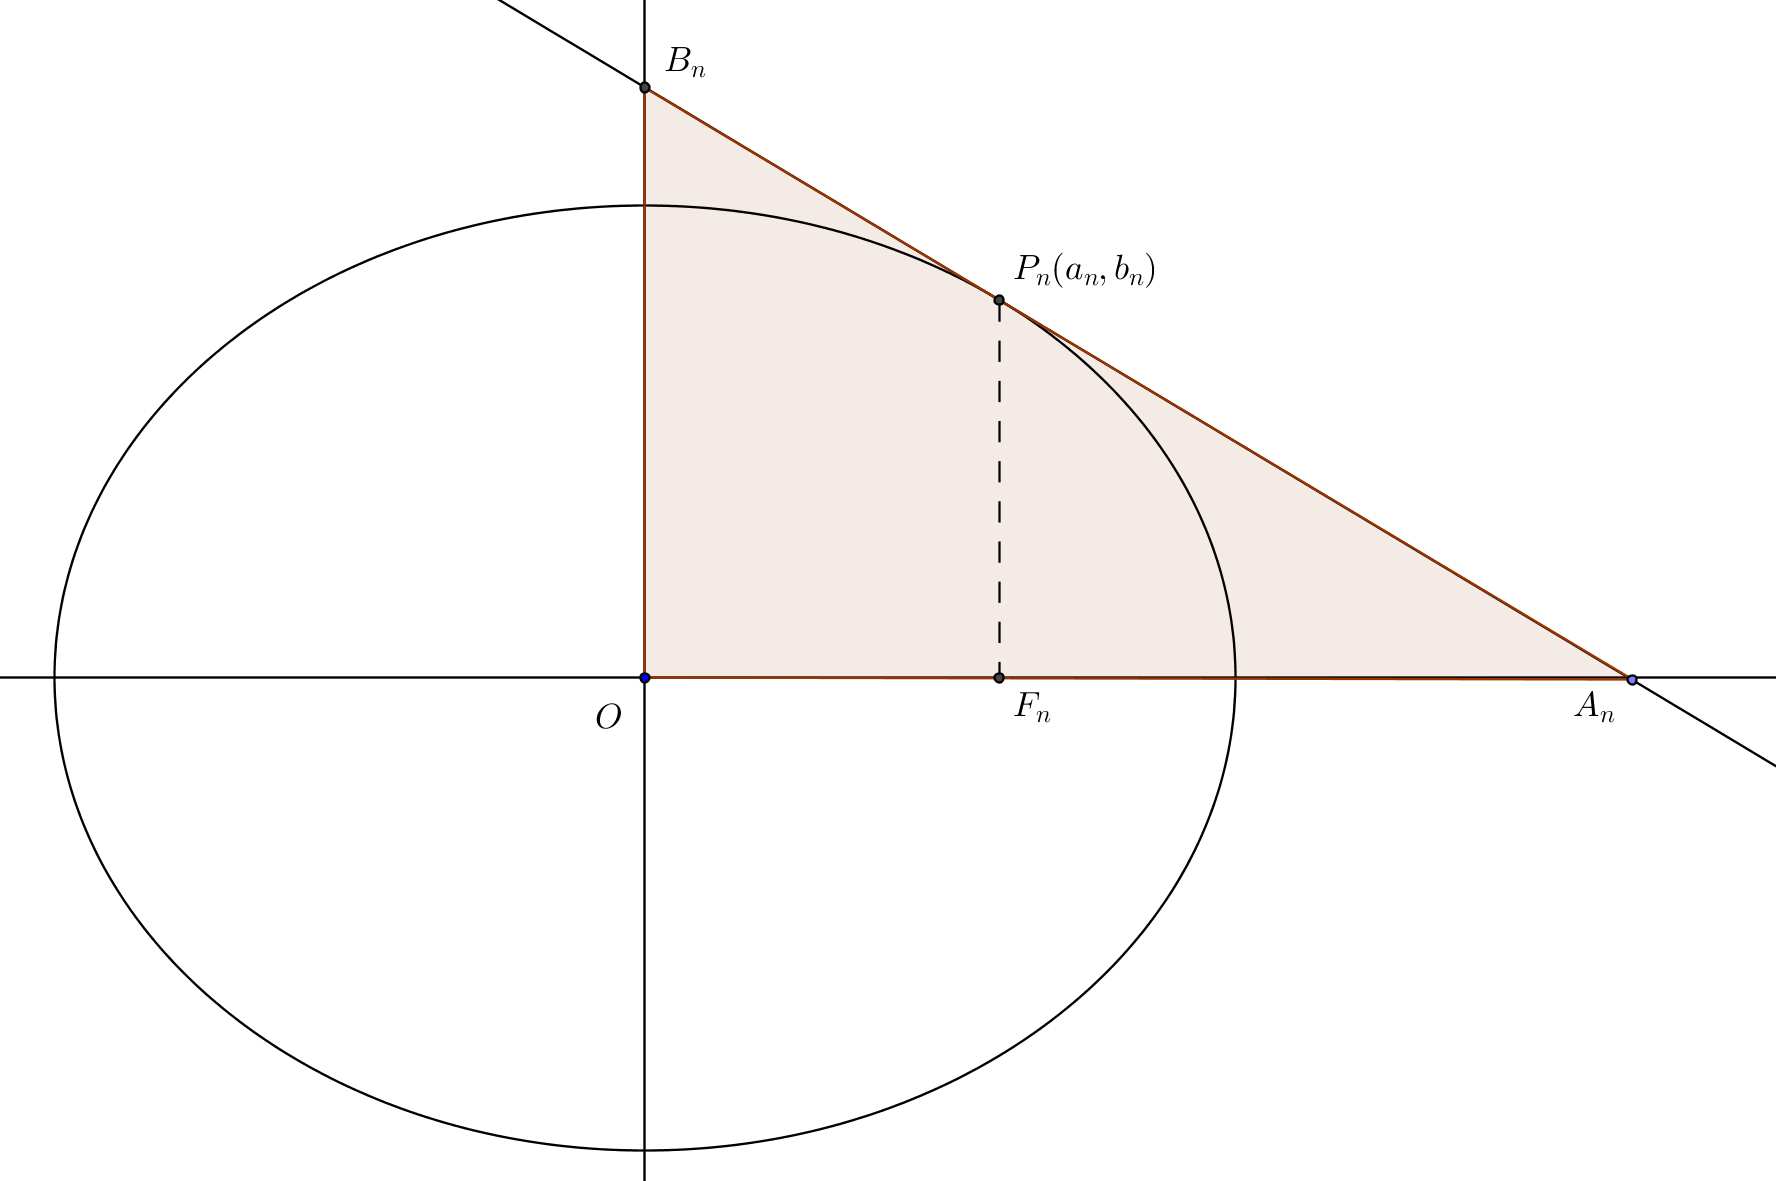
\includegraphics[width=0.9\textwidth]{01}
\end{figure}
\tabb{\(\frac18\)}{\(\frac14\)}{\(\frac12\)}{\(1\)}{\(2\)}
\newpage

%
\prob{03-실력2}
그림과 같이 선분 \(AB\) 위의 두 점 \(O_1\), \(O_2\)에 대하여 \ov A{O_1}=\ov{O_1}{O_2}=\ov{O_2}B=1일 때, 두 선분 \(AO_2\), \(O_1B\)를 각각 지름으로 하는 두 반원의 호 \(AO_2\), \(O_1B\)가 만나는 점을 \(C\)라고 하자.
호 \(O_2C\) 위를 움직이는 점 \(P\)와 호 \(O_1C\) 위를 움직이는 점 \(Q\)에 대하여 \(|\ve{O_1}P+\ve{O_2}Q|\)의 최댓값을 \(M\), 최솟값을 \(m\)이라고 할 때, \(Mm\)의 값은?
\begin{figure}[h!]
\centering
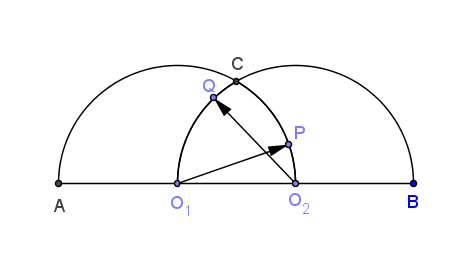
\includegraphics[width=0.5\textwidth]{02}
\end{figure}
\tabb{-1}{-\(\frac12\)}0{\(\frac12\)}1

%
\prob{04-예제1-1}
그림과 같이 삼각형 \(ABC\)에서 변 \(AB\)의 중점을 \(M\)이라 하고, 선분 \(CM\)을 4:3으로 내분하는 점을 \(D\)라고 하자.
\(\ve BD=m\ve AB+n\ve AC\)를 만족시키는 두 실수 \(m\), \(n\)에 대하여 \(m+n\)의 값은?
\begin{figure}[h!]
\centering
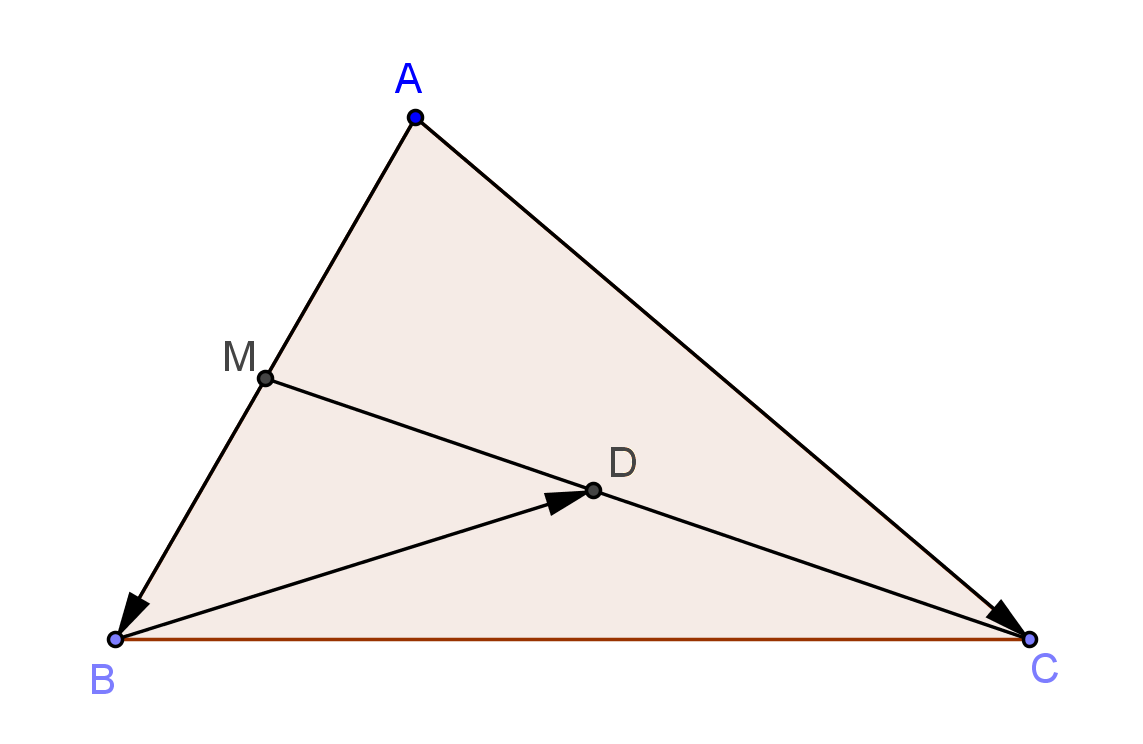
\includegraphics[width=0.5\textwidth]{03}
\end{figure}
\tabb{\(-\frac27\)}{\(-\frac3{14}\)}0{\(\frac3{14}\)}{\(\frac27\)}
\newpage

%
\prob{04-예제1-2}
그림과 같이 삼각형 \(ABC\)에서 선분 \(AB\)를 2:1로 내분하는 점을 \(D\)라고 하고, 선분 \(CD\)의 중점을 \(M\)이라고 하자.
\(\ve BM=m\ve AB+n\ve AC\)를 만족시키는 두 실수 \(m\), \(n\)에 대하여 \(m+n\)의 값은?
\begin{figure}[h!]
\centering
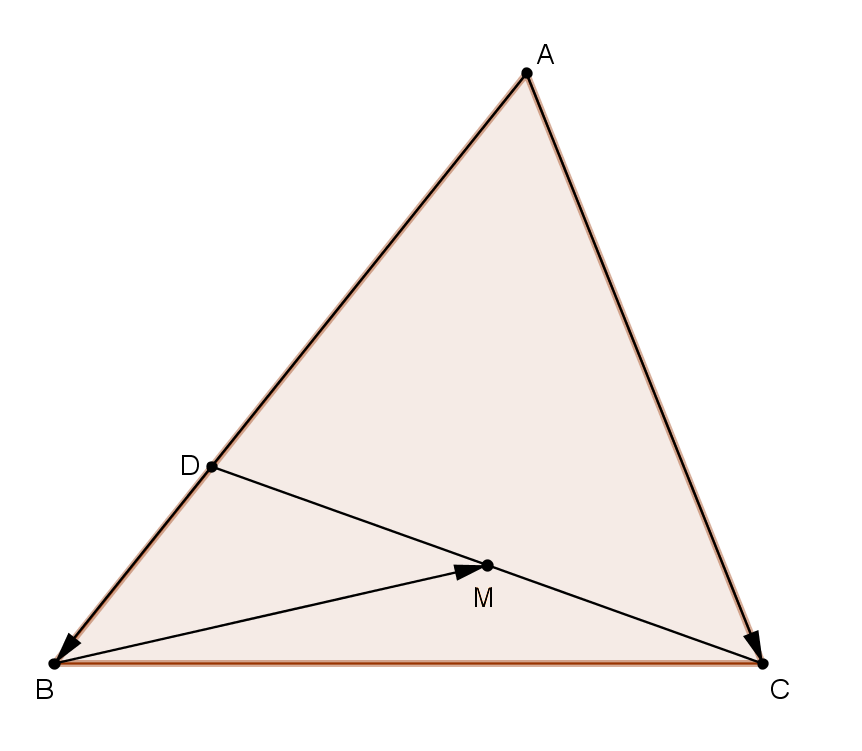
\includegraphics[width=0.5\textwidth]{03a}
\end{figure}
\tabb{\(-\frac13\)}{\(-\frac16\)}0{\(\frac16\)}{\(\frac13\)}

%%
%\prob{04-유제4}
%두 벡터 \(\vec a=(1,2)\), \(\vec u=(-1,1)\)에 대하여 벡터 \(\vec p\)를 \(\vec p=\vec a+t\vec u\)라고 하자.
%\(0\le t\le 1\)인 임의의 실수 \(t\)에 대하여 벡터 \(\vec p\)의 크기의 최댓값을 \(M\), 최솟값을 \(m\)이라고 할 때, \(\frac mM\)의 값은?
%\tabb{\(\frac23\)}{\(\frac{\sqrt5}3\)}{\(\frac{\sqrt6}3\)}{\(\frac{\sqrt7}3\)}{\(\frac{2\sqrt2}3\)}
\newpage

%
\prob{04-예제3-1}
그림과 같이 지름이 선분 \(AB\)인 원 위의 두 점 \(P\), \(Q\)에 대하여 \ov AP=3, \ov BQ=5일 때, \(\ve AB\textbullet\ve AP+\ve AB\textbullet\ve BQ\)의 값은?(단, \(\ov AB>5\)이다.)
\begin{figure}[h!]
\centering
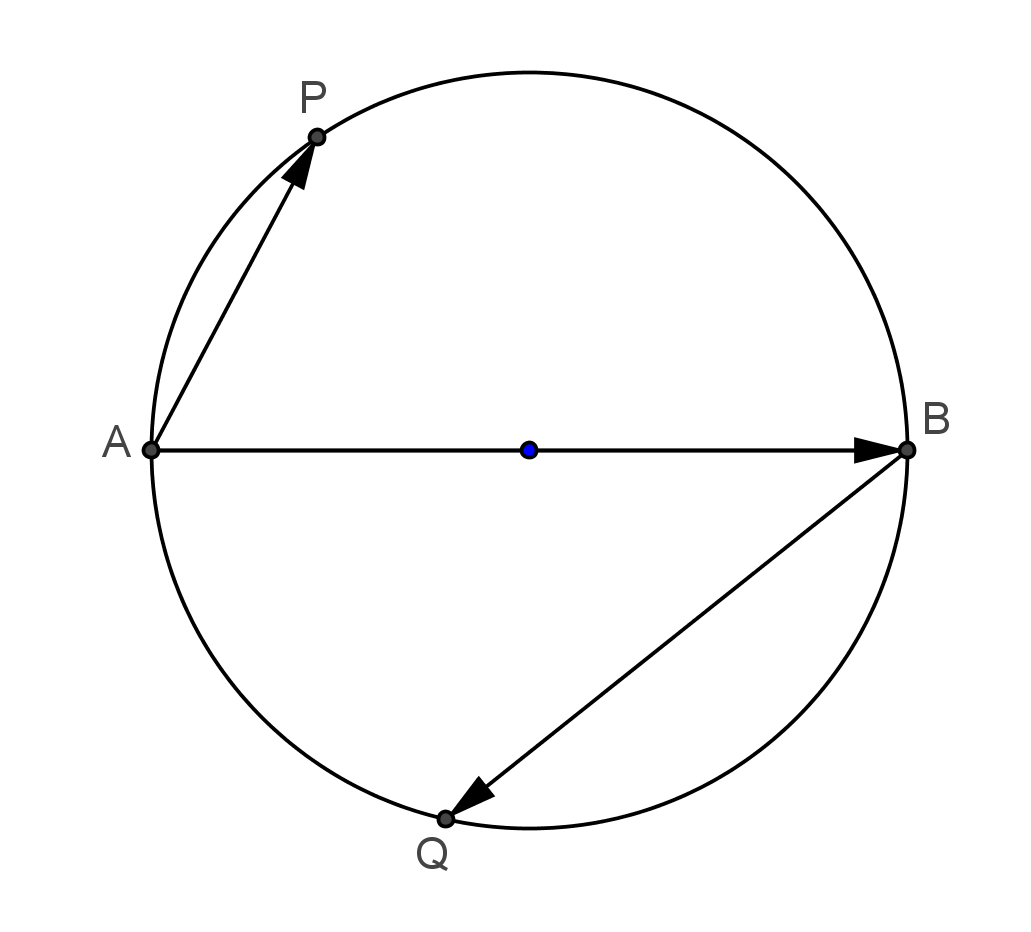
\includegraphics[width=0.45\textwidth]{04}
\end{figure}
\tabb{\(-32\)}{\(-28\)}{\(-24\)}{\(-20\)}{\(-16\)}


%
\prob{04-예제3-2}
그림과 같이 \ov BC=6, \(\angle B=\frac\pi2\)인 직각삼각형 ABC에서 \(\angle A=\theta\)라고 하자.
\(\cos\theta=\frac{2\sqrt{10}}7\)일 때, \(\ve AC\textbullet\ve AB+\ve CA\textbullet\ve CB\)의 값은?
\begin{figure}[h!]
\centering
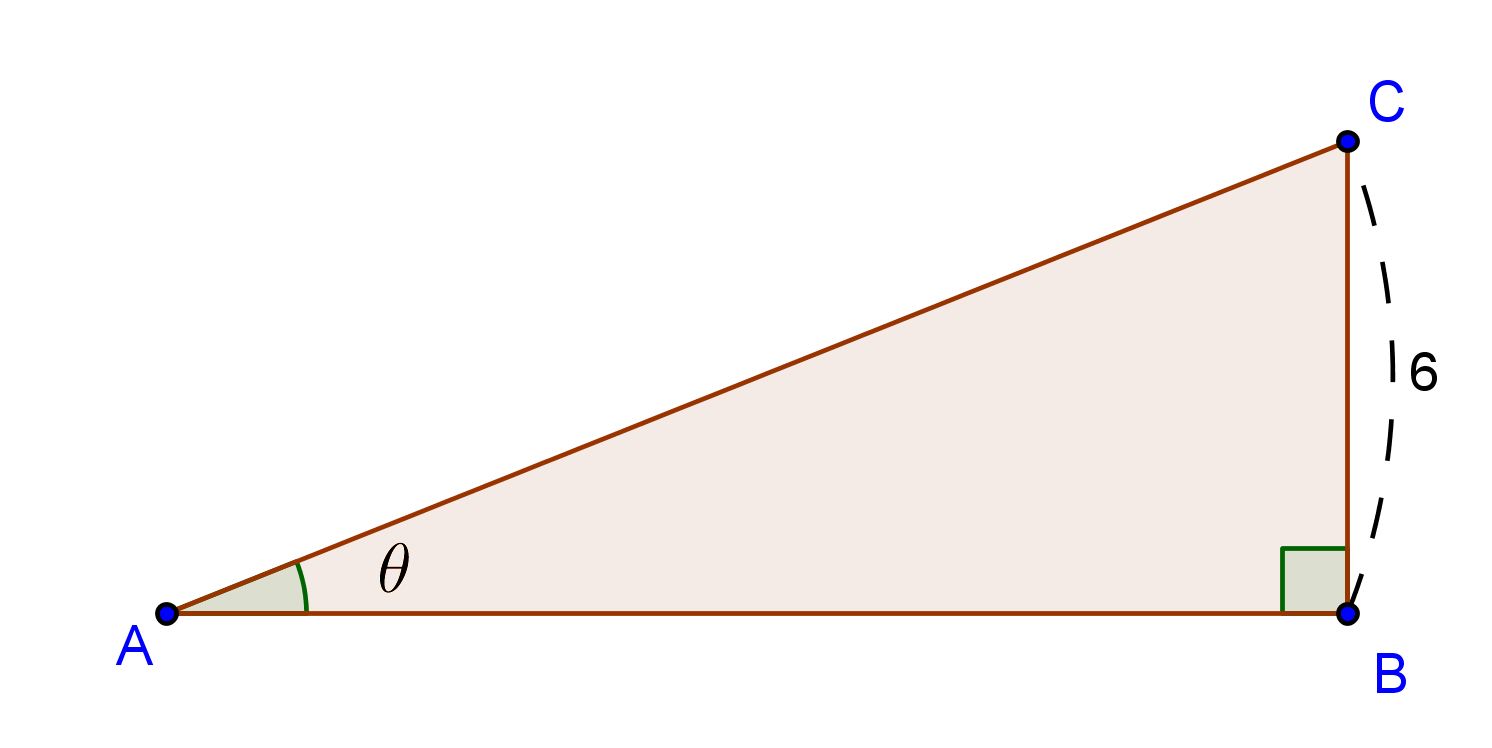
\includegraphics[width=0.45\textwidth]{05}
\end{figure}
\tabb{\(144\)}{\(169\)}{\(196\)}{\(225\)}{\(256\)}
\newpage

%
\prob{04-예제4}
세 단위벡터 \(\vec a\), \(\vec b\), \(\vec c\)가 \(\vec a+\vec b+\vec c=\vec 0\)을 만족시킨다.
두 벡터 \(\vec a\), \(\vec b\)가 이루는 각의 크기를 \(\theta\)라고 할 때 \(\cos\theta\)의 값은?
\tabb{\(-1\)}{\(-\frac{\sqrt3}2\)}{\(-\frac{\sqrt2}2\)}{\(-\frac12\)}{\(0\)}

%
\prob{04-예제8}
한 변의 길이가 3인 정삼각형 \(ABC\)에 대해 \(M\)은 선분 \(AB\)의 중점이고 \(\vec a=\ve AC\), \(\vec b=\ve AM\)이라고 하자.
\(\vec c=\frac{\vec a}{|\vec a|}+\frac{\vec b}{|\vec b|}\)일 때, \(|\vec c|\)의 값은?
%\begin{figure}[h!]
%\centering
%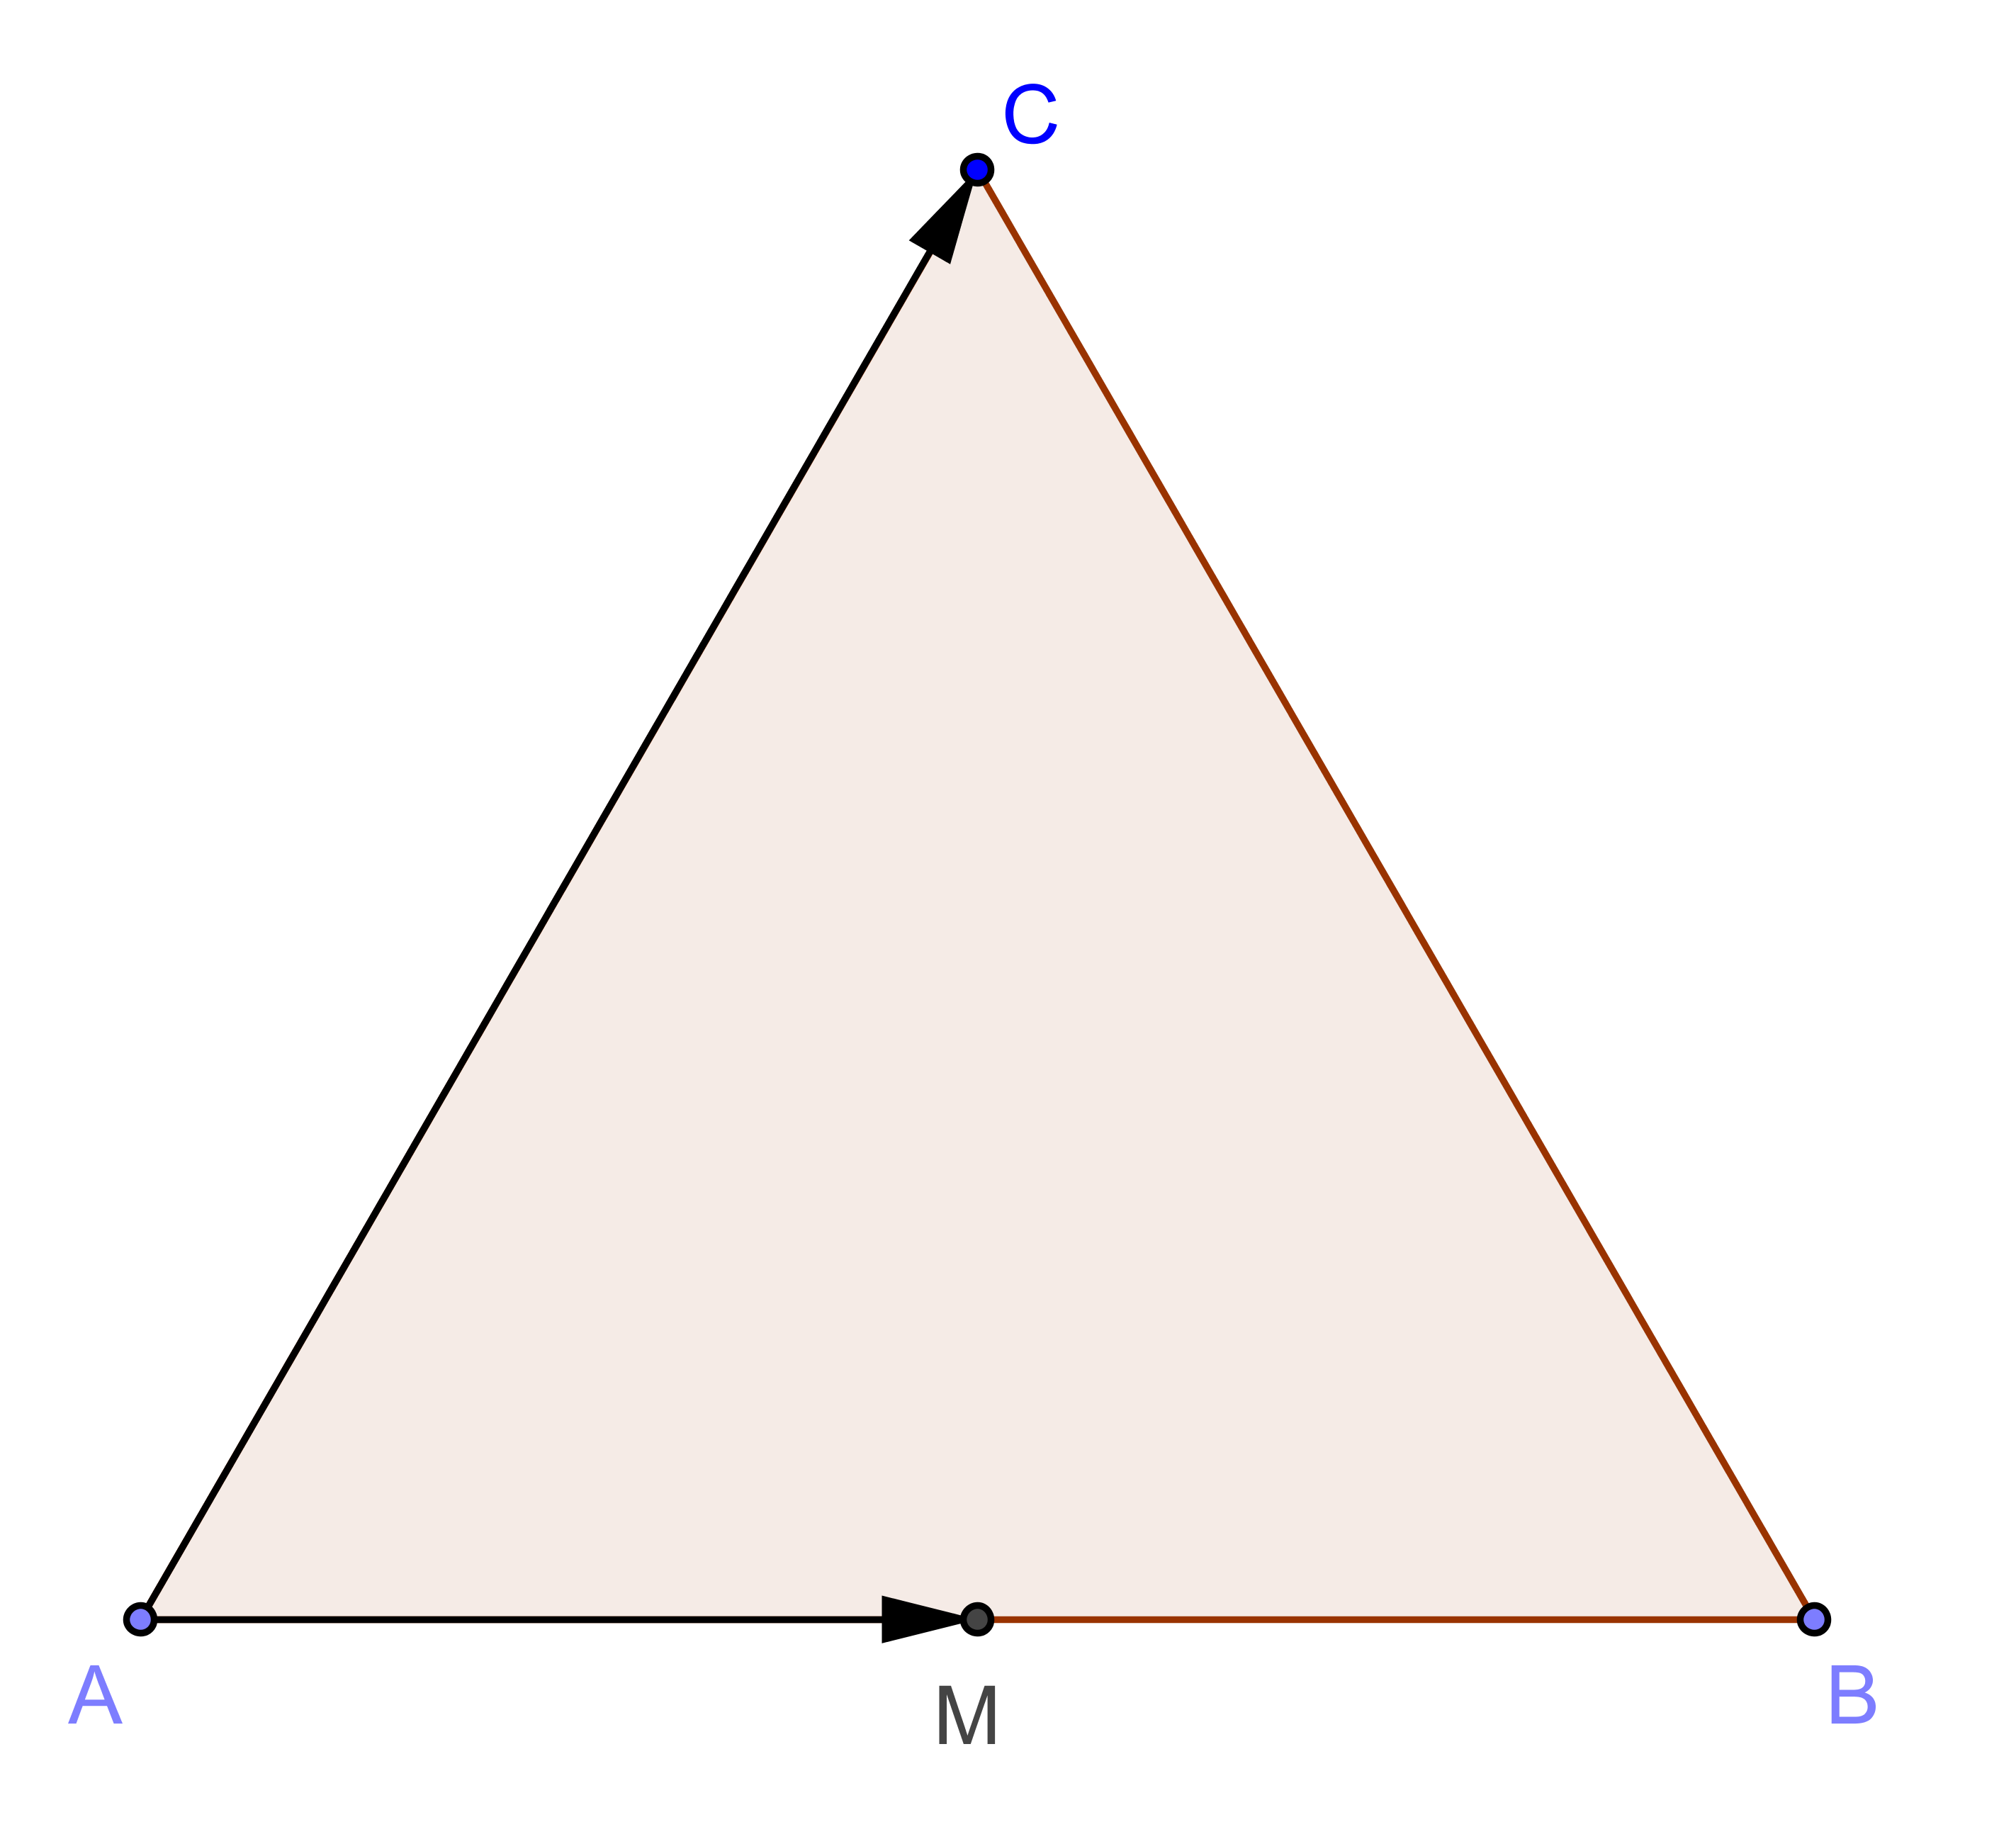
\includegraphics[width=0.4\textwidth]{06}
%\end{figure}
\tabb{1}{\(\sqrt2\)}{\(\sqrt3\)}{\(2\)}{\(\sqrt5\)}
%
%%
%\prob{04-기초1}
%삼각형 \(ABC\)의 무게중심을 \(G\), 선분 AC의 중점을 \(M\)이라고 할 때, \(\ve MG=p\ve AB+q\ve AC\)를 만족시키는 두 실수 \(p\), \(q\)에 대하여 \(p+q\)의 값은?
%\begin{figure}[h!]
%\centering
%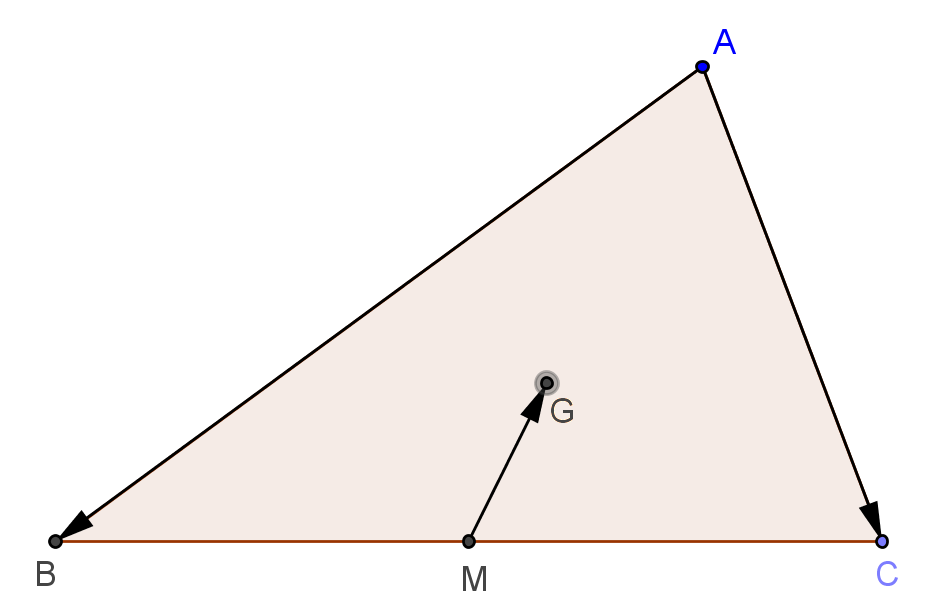
\includegraphics[width=0.5\textwidth]{07}
%\end{figure}
%\tabb{\(-\frac13\)}{\(-\frac16\)}0{\(-\frac16\)}{\(-\frac13\)}

%
\prob{04-기초3}
두 벡터 \(\vec a=(k,1)\), \(\vec b=(k-2,-3)\)가 서로 수직일 때, \(k\)의 값은?
(단 \(|\vec a|\neq|\vec b|\)이다.)
\tabb{\(-3\)}{\(-1\)}{\(1\)}{\(3\)}{\(5\)}

%
\prob{04-기초5}
좌표평면에서 두 직선 \(\frac{x+1}9=\frac y2\), \(\frac{x-4}7=\frac{y-2}6\)가 이루는 각의 크기를 \(\theta\)(\(0\le\theta\le\frac\pi2\))라고 할 때, \(\cos\theta\)의 값은?
\tabb{-\(\frac1{17}\)}{\(\frac3{17}\)}{\(\frac7{17}\)}{\(\frac{11}{17}\)}{\(\frac{15}{17}\)}
\newpage

%
\prob{04-기본1}
그림과 같이 \ov AB=4, \ov BC=9, \ov CA=8인 삼각형 ABC의 내접원의 중심을 \(P\)라고 하자.
\(\ve AP=m\ve AB+n\ve AC\)를 만족시키는 두 실수 \(m\), \(n\)에 대하여 \(m-n\)의 값은?
\begin{figure}[h!]
\centering
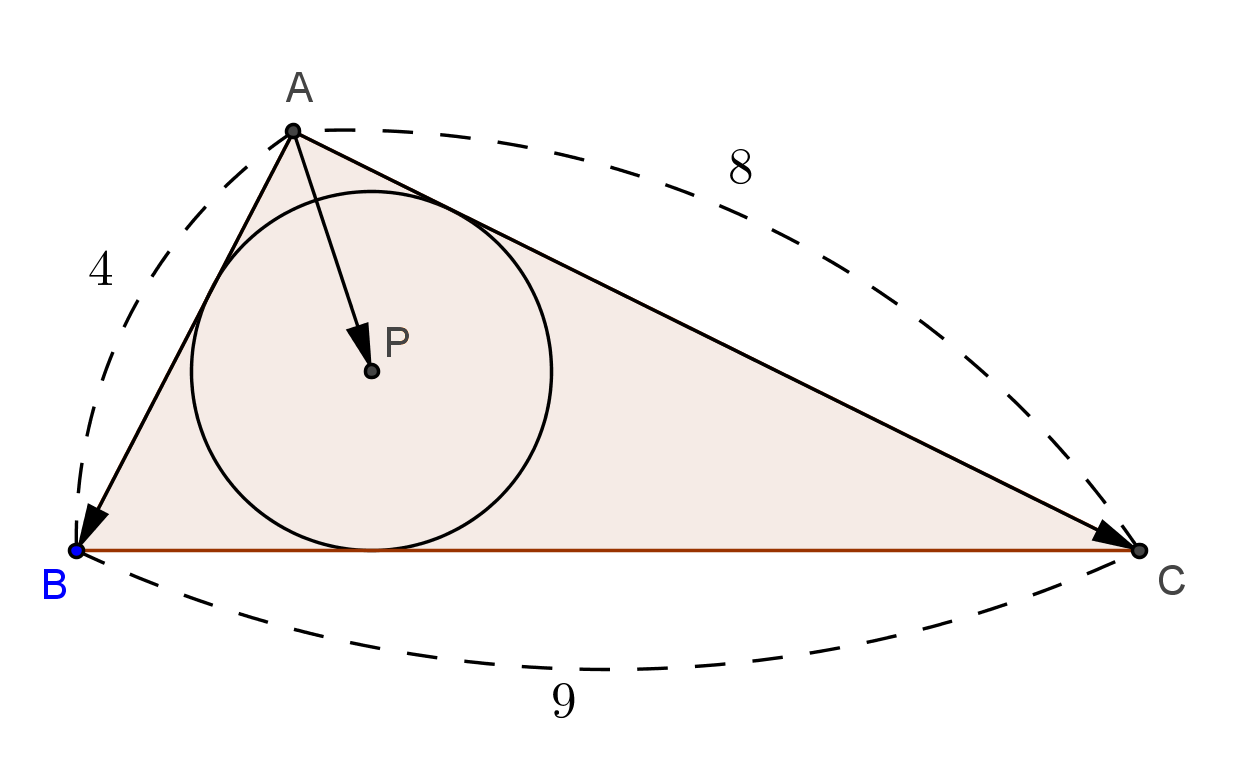
\includegraphics[width=0.6\textwidth]{08}
\end{figure}
\tabb{\(\frac17\)}{\(\frac4{21}\)}{\(\frac5{21}\)}{\(\frac6{21}\)}{\(\frac13\)}

%
\prob{04-기본2}
그림과 같이 한 평면 위에 길이가 2인 두 정삼각형 \(ABD\), \(BCD\)가 있다.
선분 \(AB\)의 중점을 \(M\)이라고 할 때 \(\ve DM\textbullet\ve MC+\ve BC\textbullet\ve AC\)의 값을 구하시오.
\begin{figure}[h!]
\centering
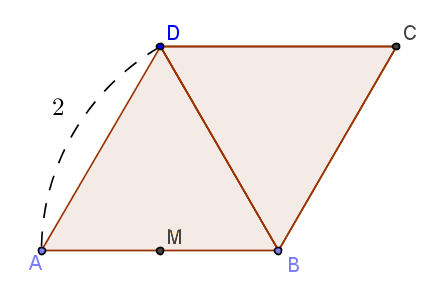
\includegraphics[width=0.5\textwidth]{09}
\end{figure}
\tabb{\(\sqrt3\)}{\(3\)}{\(3\sqrt3\)}{\(9\)}{\(9\sqrt3\)}
\newpage

%%
%\prob{04-기본3}
%세 벡터 \(\vec a=(1,1)\), \(\vec b=(0,-2)\), \(\vec c=(2n,-6)\)에 대하여 실수 \(t\)의 값에 관계없이 항상 \((t\vec a+\vec b)\textbullet(t\vec a+\vec c)+6\)의 값이 양수인 정수 \(n\)의 개수는?
%\tabb{\(11\)}{\(13\)}{\(15\)}{\(17\)}{\(19\)}

%
\prob{04-기본4}
좌표평면에서 직선 \(\frac x2=y-3\)위의 점 \(P(a,b)\)에서 \(x\)축에 내린 수선의 발을 \(Q\), \(y\)축에 내린 수선의 발을 \(R\)이라고 할 때, 직선 \(\frac x2=y-3\)와 직선 QR은 서로 수직이다.
\(a+b\)의 값은?
\tabb{\(-6\)}{\(-3\)}{\(0\)}{\(3\)}{\(6\)}

%
\prob{04-실력1-1}
선분 \(AB\) 내부의 점 \(P\)에 대하여
\[2\ve PA+\ve PB=\vec0\]
가 성립한다.
선분 \(AB\)의 길이가 12일 때, 선분 \(AP\)의 길이를 구하시오.
\tabb{\(1\)}{\(2\)}{\(3\)}{\(4\)}{\(6\)}

%
\prob{04-실력1-2}
선분 \(AB\) 내부의 점 \(P\)에 대하여
\[3\ve AP+5\ve BP=\vec0\]
가 성립한다.
선분 \(AB\)의 길이가 24일 때, 선분 \(AP\)의 길이를 구하시오.
\tabb{\(3\)}{\(6\)}{\(9\)}{\(12\)}{\(15\)}
\newpage

%
\prob{04-실력1-3}
삼각형 \(ABC\)의 내부의 한 점 \(P\)에 대하여
\[3\ve PA+2\ve PB+\ve PC=\vec0\]
가 성립한다.
삼각형 \(ABP\)의 넓이가 2일 때, 삼각형 \(ABC\)의 넓이를 구하시오.
\tabb{\(4\)}{\(8\)}{\(12\)}{\(16\)}{\(20\)}

%
\prob{04-실력1-4}
삼각형 \(ABC\)의 내부의 한 점 \(P\)에 대하여
\[\ve AP+3\ve BP+4\ve CP=\vec0\]
가 성립한다.
삼각형 \(ACP\)의 넓이가 3일 때, 삼각형 \(ABC\)의 넓이를 구하시오.
\tabb{\(6\)}{\(8\)}{\(10\)}{\(12\)}{\(14\)}
\newpage

%
\prob{04-실력2}
좌표평면 위에 세 점 \(A\), \(B\), \(D\)가 있다.
두 선분 \(AD\), \(BC\)가 평행하도록 점 \(C\)를 잡을 때,
\[\ve AB=(1,-2),\quad\ve BC=(x,y),\quad\ve CD=(-5,1)\]
이다.
\ve BC=\ve OP를 만족시키는 점 \(P\)에 대하여 \(4\le x\le 8\)일 때, 점 \(P\)가 나타내는 도형의 길이는?
(단, \(O\)는 원점이고, \(xy\neq0\)이다.)
\begin{figure}[h!]
\centering
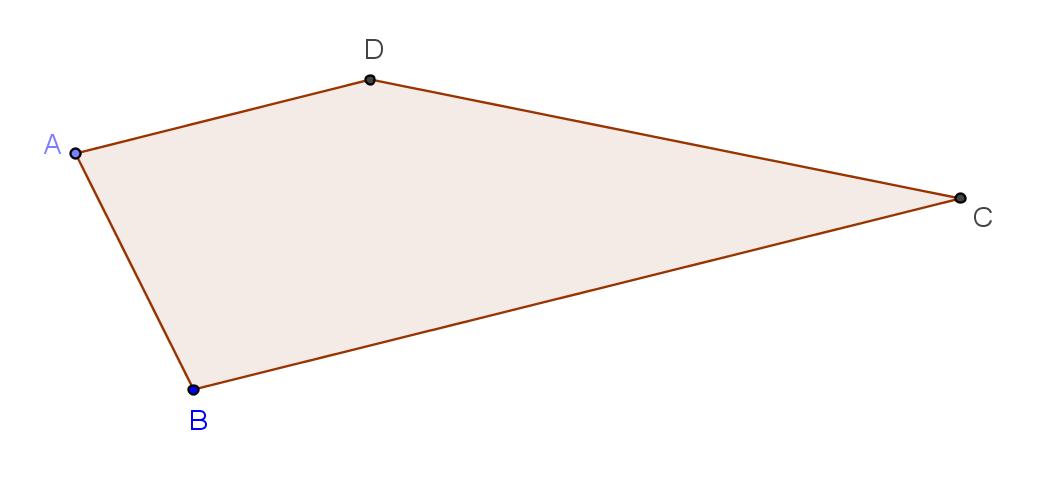
\includegraphics[width=0.7\textwidth]{10}
\end{figure}
\tabb{\(\sqrt5\)}{\(\sqrt{10}\)}{\(\sqrt{13}\)}{\(\sqrt{17}\)}{\(5\)}
\newpage

%
\prob{04-실력3}
그림과 같이 원점이 \(O\)인 좌표평면 위의 두 점 \(A(2,0)\), \(B(0,2)\)에 대하여 선분 \(AB\) 중점을 \(C\)라고 하고, \(\ve OA=\vec a\), \(\ve OB=\vec b\), \(\ve OC=\vec c\)라고 하자.
\[\vec p=\vec a+\vec c,\quad \vec q=2\vec b-\vec c\]
라고 할 때, 등식
\[|x\vec p+y\vec q|=2\sqrt{10}\]
이 성립하도록 하는 두 실수 \(x\), \(y\)의 순서쌍 \((x,y)\)를 좌표로 하는 점 \(P\)가 그리는 도형의 길이를 구하시오.
\begin{figure}[h!]
\centering
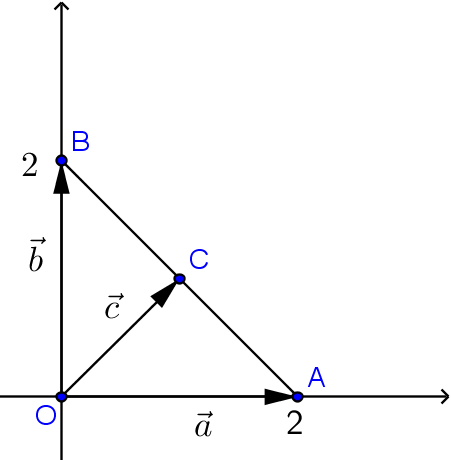
\includegraphics[width=0.3\textwidth]{11}
\end{figure}
\tabb{\(\pi\)}{\(2\pi\)}{\(3\pi\)}{\(4\pi\)}{\(5\pi\)}
\newpage

%
\prob{04-기출}
한 변의 길이가 2인 정삼각형 ABC에서 변 \(AB\)의 중점을 \(D\)라고 하고, 변 AC를 2:1과 1:2로 내분하는 점을 각각 \(E\), \(F\)라고 할 때, \(|\ve BF+\ve DE|^2\)의 값은?
\begin{figure}[h!]
\centering
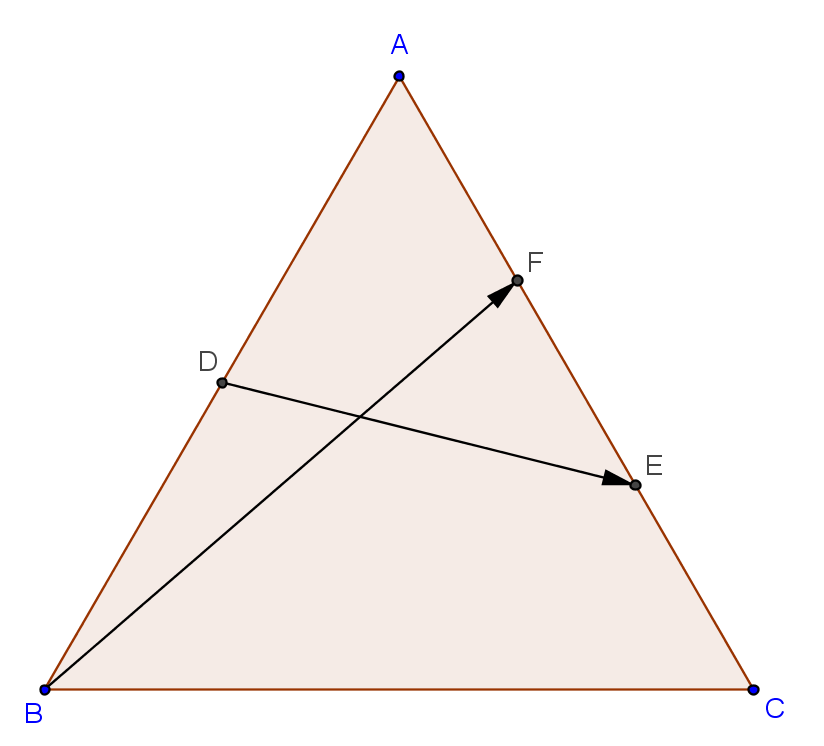
\includegraphics[width=0.5\textwidth]{12}
\end{figure}
\tabb{\(3\)}{\(4\)}{\(5\)}{\(6\)}{\(7\)}

\bigskip\bigskip\bigskip\bigskip
%%%%
\begin{table}[h!]
\begin{tabular}{|c|c||c|c||c|c||c|c|}
\hline
\pn&\ding{174}	&\pn&\ding{174}	&\pn&\ding{172}	&\pn&\ding{173}\\\hline
\pn&\ding{176}	&\pn&\ding{174}	&\pn&\ding{175}	&\pn&\ding{174}\\\hline
\pn&\ding{173}	&\pn&\ding{176}	&\pn&\ding{173}	&\pn&\ding{173}\\\hline
\pn&\ding{176}	&\pn&\ding{175}	&\pn&\ding{176}	&\pn&\ding{174}\\\hline
\pn&\ding{173}	&\pn&\ding{175}	&\pn&\ding{175}	&\pn&\ding{176}\\\hline
\end{tabular}
\end{table}

\end{document}